%%%%%%%%%%%%%%%%%%%%%%%%%%%%%%%%%%%%%%%%%%%%%%%%%%%%%%%%%%%%%%%%%%%%%%%%%%%%%%%%%%%
% Team: Rainy
% Members: Rain  Dickson  Sareddy
% Relative files:
% Note: Do not compile this file compile Main.tex to get the pdf file instead.
%%%%%%%%%%%%%%%%%%%%%%%%%%%%%%%%%%%%%%%%%%%%%%%%%%%%%%%%%%%%%%%%%%%%%%%%%%%%%%%%%%%
\subsection{Lataent Semantic Analysis}
Measuring the similarity between words, sentences, paragraphs and documents is an important component in various tasks such as information retrieval, document clustering, word-sense disambiguation, automatic essay scoring, short answer grading, machine translation and text summarization. 
This survey discusses the existing works on text similarity through partitioning them into three approaches; String-based, Corpus-based and Knowledge-based similarities. 
Furthermore, samples of combination between these similarities are presented.
Text similarity measures play an increasingly important role in text related research and applications in tasks such as information retrieval, text classification, document clustering, topic detection, topic tracking, questions generation, question answering, essay scoring, short answer scoring, machine translation, text summarization and others. 
Finding similarity between words is a fundamental part of text similarity which is then used as a primary stage for sentence, paragraph and document similarities. 
Words can be similar in two ways lexically and semantically. Words are similar lexically if they have a similar character sequence. Words are similar semantically if they have the same thing, are opposite of each other, used in the same way, used in the same context and one is a type of another. 
Lexical similarity is introduced in this survey though different String-Based algorithms, Semantic similarity is introduced through Corpus-Based and Knowledge-Based algorithms. 
String-Based measures operate on string sequences and character composition. A string metric is a metric that measures similarity or dissimilarity (distance) between two text strings for approximate string matching or comparison. 
Corpus-Based similarity is a semantic similarity measure that determines the similarity between words according to information gained from large corpora. 
Knowledge-Based similarity is a semantic similarity measure that determines the degree of similarity between words using information derived from semantic networks. The most popular for each type will be presented briefly.
 
\subsection{Metadata Extraction}
Metadata Extractor is the module which can extract metadata in PDF files such as title, subheading, doi, etc. We use python package pyPdf to extract metadata directly and use metadata to do couple things. First, we extract titles of articles returning those to the web page as search results. Second, we use metadata extractor to extract subheadings which are treated as the definition of break point to split PDF file i.e. one article will be separated into small pieces based on subheading. The small pieces will convert into .txt files by the .txt converter we built so that we can take .txt files into similarity comparison and get the most relative parts in the article.Third, We extract doi [explain what is doi] which can link to the original article source. 
      \subsection{Extracting Information from Text}
For any given question, it's likely that someone has written the answer down somewhere. The amount of natural language text that is available in electronic form is truly staggering, and is increasing every day. 
However, the complexity of natural language can make it very difficult to access the information in that text. The state of the art in NLP is still a long way from being able to build general-purpose representations of meaning from unrestricted text. 
If we instead focus our efforts on a limited set of questions or "entity relations," such as "where are different facilities located," or "who is employed by what company," we can make significant progress.
\subsection{Similarity Comparison}
	\begin{figure*}[htb]
		\begin{center}
			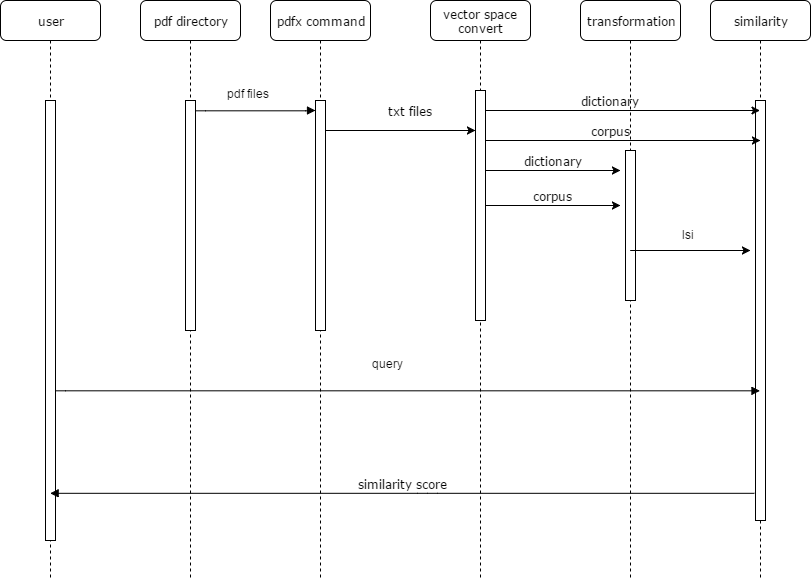
\includegraphics[width=0.8\textwidth]{Rainy_Sequence_diagram}
		\end{center}
		\caption{Sequence diagram of text similarity compare function.\label{Sequence diagram}}
	\end{figure*}
	\newpage